%!TEX root = ../thesis.tex
\chapter{Entropy Rate Estimation\label{ch:crossentropy}}

Extracting information flows is a problem deeply rooted in information theory. To examine these flows requires tools to quantify and measure this information in the form of natural language. As discussed in \autoref{ch:background}, the words used to construct language have no qualitative meaning in the context of the numerical analysis. This means that the tools are comparative in nature. Indeed, information theory has been used extensively to compare properties of information in language\todo{cite several papers, maybe add a bit more detail here}. 

In this chapter, we extend this philosophy in two key ways. We introduce a non-parametric entropy rate estimator and check it's assumptions using real data. We then generalise this entropy rate to a cross entropy rate, developing a tool for analysing information flows. 

\section{Entropy Rate Estimation}

Recall \autoref{def:entropyrate} of the entropy rate of a stochastic process. While a useful theoretical tool, this can be very difficult to compute, requiring knowledge of the joint entropy for a infinite set of realisations.

To overcome this, we seek a way to estimate the entropy of the process from a known sequence of data. In 1998 Kontoyianni et al. proved the convergence of a non-parametric entropy estimator in stationary processes~\cite{kontoyiannisNonparametricEntropyEstimation1998}.

\begin{definition}[Kontoyianni Entropy Rate] \label{def:kontoyianni}
	For a stochastic process $\mathcal{X} = \{X_i\}$, with $n$ realisations, the entropy rate is given by,
	\begin{equation}\label{eq:entropy:kontoyiannidef}
		H(\mathcal{X}) = \lim_{n\to \infty}\frac{n \log n }{\sum_{i=0}^n \Lambda_{i} },
	\end{equation}
	where  $\Lambda_{i}$ is the length of the shortest subsequence starting at position $i$ that does not appear as a contiguous subsequence in the previous $i$ symbols $X_{0}^{i}$. This can also be obtained by adding 1 to the longest match-length, 
	 \begin{equation}\label{eq:entropy:lambda}
	  \Lambda_{i}=1+\max \left\{l: X_{i}^{i+l}=X_{j}^{j+l}, 0 \leq j \leq N-i, 0 \leq l \leq N - i - j \right\}.
	 \end{equation}
\end{definition}

%<lit review>
This idea of using matched sub-sequences of text draws from the original work by Lempel and Ziv~\cite{zivUniversalAlgorithmSequential1977} in compression algorithms based on coding schemes. These algorithms attempt to compress a sequence down into the smallest possible representation, which at perfect efficiency would be the entropy, $H$. However these universal coding algorithms have no universal rate of convergence~\cite{shieldsUniversalRedundancyRates1993, shieldsUniversalRedundancyRates1995} and in practice other approaches are often employed, tailored to the specific application at hand.

The idea of an entropy estimator based on match lengths was originally put forward by Grassberger~\cite{grassbergerEstimatingInformationContent1989} and proved consistent for independent and identically distributed (i.i.d.) processes and mixing Markov chains~\cite{shieldsEntropyPrefixes1992}, stationary processes~\cite{kontoyiannisPrefixesEntropyRate1994} and more generally to random fields~\cite{quasEntropyEstimatorClass1999}.


Wyner and Ziv~\cite{wynerAsymptoticPropertiesEntropy1989} showed that for every ergodic process the match length $\Lambda_{n}$ grows like $\frac{\log{n}}{H}$ in probability.  Extending from this notion Kontoyianni et al. showed the convergence of \autoref{eq:entropy:kontoyiannidef} in stationary ergodic processes using the match-length $ \Lambda_{i}$. This match-length in \autoref{eq:entropy:lambda} can be seen as the length of the next phrase to be encoded in the sliding-window Lempel–Ziv algorithm.

%<match lengths>
Conceptually, this match-length is simple. \autoref{fig:entropy:matchlength} show the calculation of two match-lengths at different time points of a line from Doctor Seuss. At each index $i$, the elements immediately proceeding ($i, i+1, i+2, \dots$) are compared to the history of elements before $i$. The matches of length $k$ are found such that the elements from $j$ to $j+k$ perfectly match the elements from $i$ to $i+k$, for any $j<i$ where $k$ is then maximised. This search only considers the length of the match, regardless of it's location in the history. 

\begin{figure}[hb]
	\centering
	\includestandalone[width=\textwidth]{chapter2/figs/tikz/lambda_count}
	\caption{An example calculation of the match-length based $\Lambda_i$ applied to a line from Green Eggs and Ham by Doctor Seuss. {\color{blue} Blue text} is that which has been matched from past to the future.\label{fig:entropy:matchlength}} 
\end{figure}
%</match lengths>

Even before it's formalisation by Kontoyianni et al., similar estimators had appeared in the literature applied to experimental data to determine the entropy rates of processes~\cite{chenUsingDifficultyPrediction1993, chenFastPatternMatching1995, farachEntropyDNAAlgorithms1995, juolaWhatCanWe1997}.
%</lit review>

% Final note
Moving forward we will assume any any discussion of the \emph{entropy rate} of a single process is assumed to be the \emph{Kontoyianni entropy rate} of that process, unless otherwise stated.


% ASSSUMPTIONS
\section{Assumptions of Entropy Rate Estimation}

The proof of convergence of this entropy rate places some limits on the process of investigation. In particular, three assumptions are made for convergence: ergodicity, stationarity and the Doeblin Condition (DC).

The Doeblin Condition is a reasonably weak condition, but is fundamental in the proof of the convergence. Simply put, the DC requires that after an arbitrary $r$ time steps, every state is possible again with positive probability~\tocite{Konto Prefixes and the entropy rate for long-range sources}. More formally, the definition is as follows.

\begin{definition}[Doeblin Condition (DC)]
	There exists an integer $r\geq 1$ and a real number $\beta \in(0,1)$  such that,  for all  $x_{0} \in \mathcal{A}, \quad P\left\{X_{0}=x_{0} \mid X_{-\infty}^{-r}\right\} \leq \beta, $ with probability one. 
\end{definition}

Fortunately, as Kontoyianni et al. themselves state, the DC is ``certainly satisfied by natural languages''~\cite{kontoyiannisNonparametricEntropyEstimation1998}. Given the DC is not a fierce restriction condition is assumption is easy to satisfy. 

In contrast, the assumptions of ergodicity and stationarity are  harder to confirm. A long-standing assumption of information theory is that natural language can be modelled by a stationary process~\tocite{Shannon, A mathematical theory of communication.  Prediction and entropy of printed English, Cover, T.M.; Thomas, J.A. Elements of Information Theory}. The assumption, while flawed, is well precedented and used again in this work.

While the much of the literature including the work of Kontoyianni assume ergodicity of natural language, some suggest that language should be modelled by a \emph{strongly nonergodic} stationary process~\cite{debowski_is_2018}. In brief, this contention is founded upon the idea that any given collection of text, such as a book, has a topic containing a small finite subset of words. Suggesting that it's text will inherently not explore the full state space of language. While well founded, our interest is not to look at the entropy rate of the English language as a whole, but rather to look at the entropy rate of individual text streams, which can explore the state space of news under consideration. As such, the assumptions of ergodicity and stationarity appear justified in the context of the problem.


%<Convergence>
\subsubsection{Convergence}
With the assumptions of the proof addressed, the challenges of entropy convergence needs to be examined. The entropy rate defined in \autoref{eq:entropy:kontoyiannidef} is based upon an infinite set of both data to calculated $\Lambda_i$'s over. In reality, we have finite data, and need to examine the convergence of a modified estimator.

\begin{definition}[Kontoyianni Entropy Rate Estimator] \label{def:kontoyianni}
	The Kontoyianni Entropy Rate in \autoref{def:kontoyianni} can be estimated on a finite stochastic process $\mathcal{X} = \{X_i\}$, with $N$ realisations, by
	\begin{equation}\label{eq:estimate}
		\hat{h} = \frac{N \log N }{\sum_{i=0}^n \Lambda_{i} },
	\end{equation}
	where  $\Lambda_{i}$ is the length of the shortest subsequence starting at position $i$ that does not appear as a contiguous subsequence in the previous $i$ symbols $X_{0}^{i}$.
	 \begin{equation}
	  \Lambda_{i}=1+\max \left\{l: X_{i}^{i+l}=X_{j}^{j+l}, 0 \leq j \leq N-i, 0 \leq l \leq N - i - j \right\}.
	 \end{equation}
\end{definition}

To examine the convergence of the estimator, a model of language can be used to generate sequences of text, upon which we can estimate the entropy rate.

%<Zipf convergence>
\begin{figure}[h]
\centering
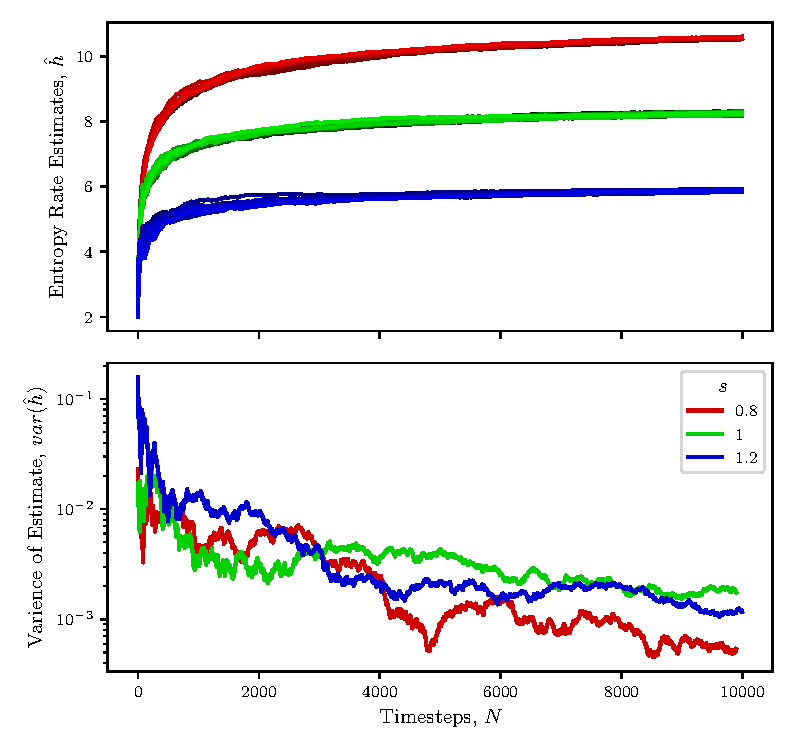
\includegraphics{chapter2/figs/Zipf_entropy_convergence.pdf}
\caption{Convergence of the Kontoyianni entropy rate estimator on sequences of i.i.d Zipf law realisations with varying Zipf law rates, $s$. \label{fig:entropy:zipfconvergence}}
\end{figure}


\autoref{fig:entropy:zipfconvergence} shows the convergence of the estimator for a set of i.i.d realisations of a Zipf's law distribution. As discussed in \autoref{sec:textgeneration}, Zipf's law is a common tool for generating simple text due to it's similarity to the power-law distributions of vocabulary seen in real corpora. The Zipf's law can be used with a number of exponents, $s$, where larger exponents tighten the distribution, reducing the observed vocabulary size of the sequence and hence the entropy. 

Sequences are generated with 20,000 i.i.d realisations of the Zipf's law and the entropy rate estimated of a process is estimated at each timestep between 1 and 20,000. Estimates of entropy start very low when few realisations are available and rapidly rise as new realisations add complexity. Within the first few hundred timesteps entropies estimates can vary as new realisations are added matching or not-matching previous realisations. This is reflected in the high variance between entropies estimates for Zipf process with the same exponent in these early stages. As the number of timesteps included reaches 5000 to 7500 the bias and variance of the estimate are significantly reduced and begin plateauing.

As more timesteps are added, the estimator continues to converge to the asymptotic entropy and the variance between estimates continues to reduce. High complexity sequences take longer to converge to this entropy, but achieve suitably small levels of bias and variance within 700 timesteps. This is an important finding given the speed of calculating these estimates. The algorithm of calculated the match-lengths needed for estimating the entropy is $O(n^3)$ time complexity. As a result, speed takes a significant hit as the number of timesteps is increases. When performing simulations a parsimonious choice of simulation length is advantageous in allowing multiple simulations to be run. Hence, for Zipf law distributions a simulation length of 10000 is deemed sufficient for convergence to the entropy.
%</Zipf convergence>


%<Zipf real entropy>
To confirm the validity of this approach, we can examine the known entropy rate of the Zipf processes. As shown in \autoref{proof:iidentroptrate}, the entropy rate of an i.i.d process is simply the entropy of each element. In the case of a Zipf law the distribution has entropy\footnote{
	Proof: The probability of a word of rank $k$ being selected from a pool of $N$ elements using exponent $s$ is $(k^s H_{N,s})^{-1}$. Hence, the entropy of each individual element is $\sum_{k=1}^N  (k^s N_{N,s})^{-1} \ln\left( (k^s N_{N,s})^{-1} \right)$. Using $H_{N,s} = \sum_{k=1}^N \frac{1}{k^s}$, this can be rearranged to $\frac{s}{H_{N, s}} \sum_{k=1}^{N} \frac{\ln (k)}{k^{s}}+\ln \left(H_{N, s}\right)$. }, 
\begin{equation}
	\frac{s}{H_{N, s}} \sum_{k=1}^{N} \frac{\ln (k)}{k^{s}}+\ln \left(H_{N, s}\right)
\end{equation}
where $H_{N,s}$ is the Nth generalized harmonic number defined by, $H_{N,s} = \sum_{k=1}^N \frac{1}{k^s}$. Using an exponent of $s=1.5$ and $N$ set to the integer limit of the computer ($2^{31}$), this entropy rate is \emph{3.21755}. However, using $\lim_{N\to \infty} H_{n,s} = \zeta(s)$ and computing $\sum_{n=1}^{\infty} \frac{\log (n)}{n^{1.5}}\approx 3.93224$, we can approximate the asymptotic entropy rate as \emph{3.21811}. These are sufficiently similar and we refer to the later as the `true entropy rate' moving forward. % Talk about appraoch here.

Using simulations of the Zipf process for a variety of values of the exponent $s$, we compare how the estimated entropy rate compares to the true entropy rate. Simulations are run for values of $s$ in the range [1.01, 2.5] with increments of 0.01. 
High values of $s$ in this range have an increasingly lower entropy, as the skewness of the distribution becomes more extreme. This distribution results in a high numbers of realisations of low rank words creating repeated sequences which lower both the analytic entropy rate and the entropy rate estimate. Values above 2.5 reduce the entropy rate in vanishingly smaller increments. 

For values of $s$ above 1.1 the entropy rate estimate appears to be a rough upper bound on the true entropy rate of the process. This upper bound is only achieved with sufficient lengths of sequences such that the estimator can converge to this upper bound. Indeed, given sufficient length the variance of the estimates on sequences drawn from the same distribution is very low. This is in contract to the bias of the estimate, which varies slightly with the changing exponent. 

When $s$ becomes lower than 1.1, the Zipf law distribution becomes more even. This results in a larger probability of low rank word occurrences, producing a process with fewer repeated words or subsequence.

the variance of the distribution explodes leading to extremely high entropies as words don't appear multiple times. As $s$ increases above two, the entropies changes incrementally smaller. %IMPROVE

\autoref{figs:entropy:convergencetotruth} show these simulations and compares the true entropy rate against the entropy rate estimate. Interestingly, the entropy rate estimate over 20,000 realisations of the Zipf processes does not converge to the analytic entropy rate. Further, this bias of the estimator is not constant and varies slightly with the entropy rate. In contrast to this varying bias, the variance of the estimate remains extremely low for all values.

As the values of $s$ approach 1, the probability of a high rank word occurring is increased. As such, the asymptotic analytical entropy rate is much higher.



\begin{figure}
\centering
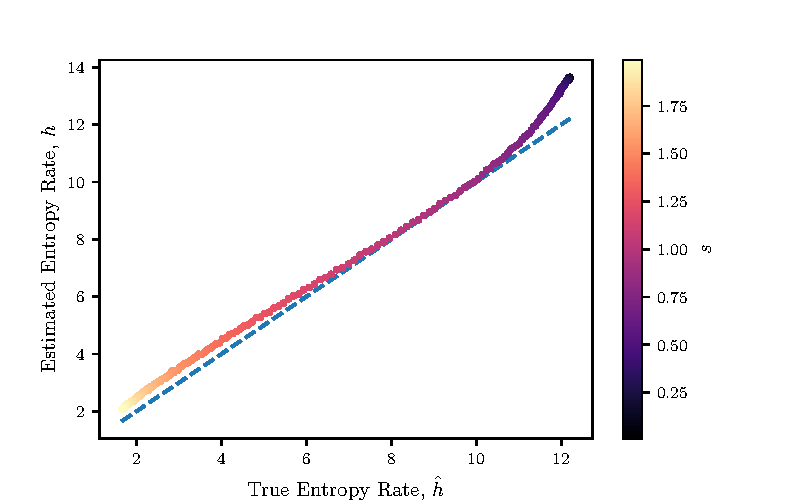
\includegraphics{chapter2/figs/convergence_to_truth.pdf}
\caption{Estimated entropy rates and analytic entropy rates of sequences of 20,000 i.i.d Zipf law random variables with exponent $s$. Dashed line represents the true entropy rate equalling the entropy rate estimate. As values for $s$ approach 0 the high variance of the distributions results in poor estimates due to the finite sample of the Zipf law. \label{figs:entropy:convergencetotruth}}
\end{figure}


%</Zipf real entropy>

%<Real data entropy convergence>
To extend from this result using the Zipf law process, we apply the same approach using the news-source Twitter data. Unlike the case of Zipf, we cannot show a true entropy rate for this distribution, but can demonstrate it's convergence.  

\begin{figure}
\centering
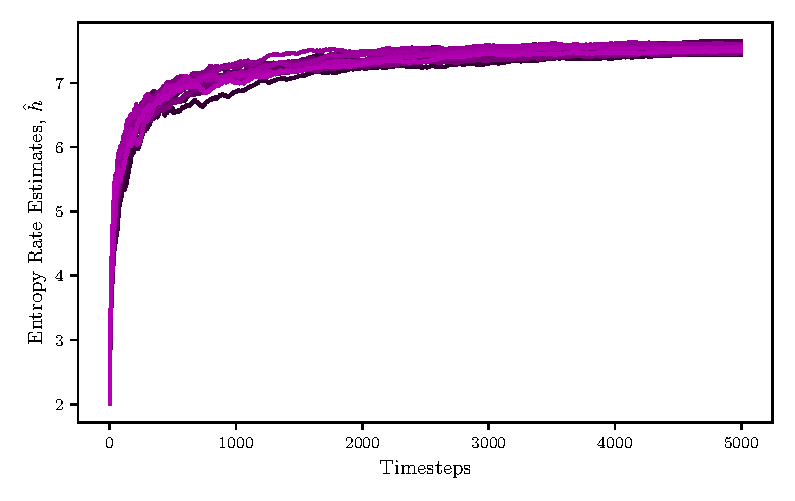
\includegraphics{chapter2/figs/real_entropy_convergence.pdf}
\caption{Convergence of the Kontoyianni entropy rate estimator on sequences words generated by drawing tweets uniformly without replacement from the pool of all tweets produced by all news-media organisations. \label{fig:entropy:realconvergence}}
\end{figure}

%</Real data entropy convergence>


%<Tikz of flow>

\begin{figure}
	\centering
	\includestandalone[width=\textwidth]{chapter2/figs/tikz/self_flow}
	\caption{Stuff} 
\end{figure}



%</Tikz of flow>



% \begin{figure}[hb]
% 	\centering
% 	\includestandalone[width=\textwidth]{chapter2/figs/tikz/window_size_change}
% 	\caption{Demonstration on window position in within data. Windows are equispaced along the entire length of data and initially non-overlapping. As the window size increases, shown in (a) $\rightarrow$ (c), the windows remain equispaced but will become overlapping. Window sizes increase until each window is almost entirely overlapping and encompasses the majority of the process. }
% \end{figure}


\section{Cross Entropy Rate}

To create a notion of information flow, we need to move beyond looking at individual sources in isolation. 



Similar to the extension of entropy, $H(X) = \sum_{x \in \mathcal{X}} p(x)\log p(x)=-\mathbb{E}[\log P(X)]$ to cross entropy, $H(p,q) = \sum_{x \in \mathcal{X}} p(x)\log $  in \autoref{def:crossentropy}, we can generalise our notion of Kontoyianni entropy rate in \autoref{def:kontoyianni} to a \emph{cross} entropy rate which we will call the Kontoyianni cross entropy rate.

\begin{definition}[Kontoyianni Full Cross Entropy Rate]
	The cross entropy rate of a {\color{target} target process} $\mathcal{T}$ coded from a {\color{source} source process} $\mathcal{S}$ can be estimated via,
	\begin{equation}
	\hat{H}(\mathcal{T} || \mathcal{S})=\frac{N_{\mathcal{T}} \log _{2} N_{\mathcal{S}}}{\sum_{i=1}^{N_{\mathcal{T}}} \Lambda_{i}(\mathcal{T}| \mathcal{S})}
	\end{equation}
	Where $\Lambda_{i}(\mathcal{T}| \mathcal{S})$ is given by the shortest subsequence starting at position $i$ in {\color{target}target} $\mathcal{T}$ that does not appear as a contiguous subsequence in the {\color{source}source} $\mathcal{S}$.
	\begin{equation}
	\Lambda_{i}(\mathcal{T}| \mathcal{S}) = \max \left\{l: T_i^{i+l}=S_{j}^{j+l}, 0 \leq j \leq N_{\mathcal{S}},  0 \leq l \leq \min( N_{\mathcal{S}}- j , N_{\mathcal{T}}- i )\right\},
	\end{equation}
	where $T_a^{b}$ and $S_a^b$ are continuous subsequences starting from index $a$ to index $b$ of the {\color{target} target}, $\mathcal{T}$, and  {\color{source} source}, $\mathcal{S}$, processes respectively.
\end{definition}

This approach is matching segments of text in the {\color{target}target} to segments of text anywhere in the {\color{source}source} in the same manner that the Kontoyianni entropy rate matched segments of text in the future of a process from a index to the history before the index. In essence, the entropy rate was asking how much information was needed on average to describe the future of a source from it's past. Comparatively, the full cross entropy rate above is taking asking how much information was needed on average to describe the {\color{target}target} given knowledge of the entire lifetime of the {\color{source}source}. \ts{Not sure how long I should keep up the colouring for.}

In the context of our problem, this estimator is cheating by viewing the future of news through the lens of the source process. As \todo{ref} illustrates, the text subsequence match in the target could be drawn from future time points in the source. This approach is interesting as it asks a simpler but very relevant question; how different are the two sources from an full information perspective.

\begin{figure}
	\centering
	\includestandalone[width=\textwidth]{chapter2/figs/tikz/unsynced_flow}
	\caption{Stuff} 
\end{figure}


While this question is interesting, and will be explored further, we need to refine this definition to help answer our question of information flow.

Rather than looking at the entire lifetime of the source during a matching calculations, we can reduce our search space to the text that occurred in the \emph{past} of the source. To achieve this we use an important piece of our data, the time that tweets occurred. For each word in the target process, $T_i$ has an associated time with it, $t(T_i)$. When matching the future of $\mathcal{T}$, starting from an index $i$, we can reduce the source process, $\mathcal{S}$ to only the words that were themselves tweeted before time $t(T_i)$. 

Put simply, we can alter the Kontoyianni full cross entropy rate to a time-synced cross entropy rate by replace the full {\color{source}} process, $\mathcal{S}$, with a time reduce source process $\mathcal{S}_{ \leq t(T_i)}$. This can be seen visually in \todo{ref tikz} and is formally defined as follows.

\begin{definition}[Kontoyianni Time-synced Cross Entropy Rate]
	The time-synced cross entropy rate of a {\color{target} target process} $\mathcal{T}$ coded from a {\color{source} source process} $\mathcal{S}$ can be estimated via,
	\begin{equation}
	\hat{H}(\mathcal{T} || \mathcal{S})=\frac{N_{\mathcal{T}} \log _{2} N_{\mathcal{S}}}{\sum_{i=1}^{N_{\mathcal{T}}} \Lambda_{i}(\mathcal{T}| \mathcal{S}_{\leq t(T_i) } )}
	\end{equation}
	Where $\Lambda_{i}(\mathcal{T}| \mathcal{S}_{\leq t(T_i) })$ is given by the shortest subsequence starting at position $i$ in {\color{target}target} $\mathcal{T}$ that does not appear as a contiguous subsequence in the time reduced {\color{source}source} $\mathcal{S}_{\leq t(T_i) }$ where,
	\begin{equation}
	\mathcal{S}_{\leq t(T_i) } = \{S_j | t(S_j) \leq t(T_i) \forall i \}.
	\end{equation}
	Which gives,
	\begin{align*}
	\Lambda_{i}(\mathcal{T}| \mathcal{S}_{\leq t(T_i)}) = \max \{l: T_i^{i+l}=S_{j}^{j+l}, 0 \leq j \leq N_{\mathcal{S}},  \\  0 \leq l \leq \min( N_{\mathcal{S}}- j , N_{\mathcal{T}}- i ) \},
	\end{align*}
	where $T_a^{b}$ and $S_a^b$ are continuous subsequences starting from index $a$ to index $b$ of the {\color{target} target}, $\mathcal{T}$ process, and the time reduced {\color{source} source}, $\mathcal{S}_{\leq t(T_i)}$, respectively.
\end{definition}
 
% Informantion flow idea
This time-synced entropy rate is testing not just the differences in the language processes of the source and target, but also measuring what information in the target is present in the source's history. This is an important distinction, as it allows us to probe a very important aspect of our data, namely, the time in which news is created. 

If a piece of information appears earlier in the source than in the target, it will be detected during the match length search, resulting in a lower entropy. This is to say, in the context of news, if the {\color{source}source} breaks a story first, \emph{less} information is required to describe the subsequent news output from the {\color{target}target}. 

Conversely, if a {\color{target}target} produces a piece of information before the {\color{source}source}, then that information will not appear in the history of the time-synced source during the match-length search. This will result in lower values of $\Lambda_i$ for that piece of information, which raises the cross entropy rate.

From this, we can find that, on average, if a {\color{source}source} produces information earlier than a {\color{target}target}, the cross entropy rate, $\hat{H}(\mathcal{T} || \mathcal{S})$, will be lower than if the {\color{target}target} produces information earlier than the {\color{source}source}. This method of examining who produces information first can be extended into a notion of \emph{information flow}, a discussion we will leave for \autoref{ch:information_flow}.


\begin{figure}
	\centering
	\includestandalone[width=\textwidth]{chapter2/figs/tikz/timesynced_flow}
	\caption{Stuff} 
\end{figure}


\todo{we can extend this with predictability}
\subsection{Validating the Assumptions Cross Entropy Estimation}
legth vs cross entropy


% test what suffiently long means in complexity ( plot of complexity vs speed of convegence)


\subsection{A Note on Package Development}

I'm thinking of putting a section here that just talks about the need for speed of computation and highlights some of the tricks used to speed it up. E.g. Fowler–Noll–Vo hashing, JIT compiling. Do you think this is appropriate to include and if so at what level of detail. 

% \subsubsection{Hashing Tokens}



\begin{figure}[h]
\centering
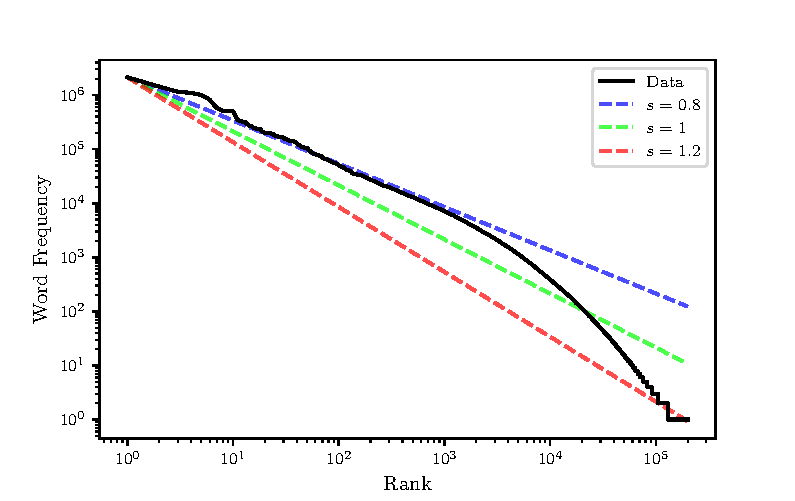
\includegraphics{chapter1/figs/fitted_zipf.pdf}
\caption{\ts{Bonus: Included for your reviewing, this is a figure that will soon be added to the data chapter.}  Word frequency of tokens in the corpus of all tweets produced by all news sources compared the rank of the token by frequency. Zipf law distributions are also shown for varying exponents, $s$. \label{fig:data:fitted_zipf}}
\end{figure} 

